\section{Qualitative Results}
Figure~\ref{fig:dcd_showcase} shows representative qualitative examples of
DCD against four baselines.  Each row corresponds to one dataset, whose name
is shown at the left.  The first column shows the raw input image, and each
remaining column shows one method\'s prediction as an error map: white denotes
true positives, red outlines false negatives, and green outlines false
positives.  The yellow insets magnify the same
local region in each prediction column.  The examples are illustrative; full
per-dataset results are in the main table.

\begin{figure}[t]
\centering
\setlength{\tabcolsep}{0.75pt}
\offinterlineskip
\renewcommand{\arraystretch}{0}
\newlength{\PW}\setlength{\PW}{0.153\columnwidth}
\newlength{\LabelW}\setlength{\LabelW}{10pt}
\begin{tabular}{@{}c*{6}{c}@{}}
\makebox[\LabelW][c]{\rotatebox{90}{\scriptsize DCA1}} & 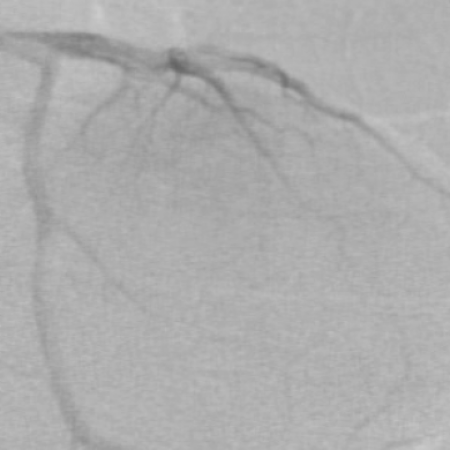
\includegraphics[width=\PW]{../img/dcd_fig6/fig5x6/r01_gt.pdf} & 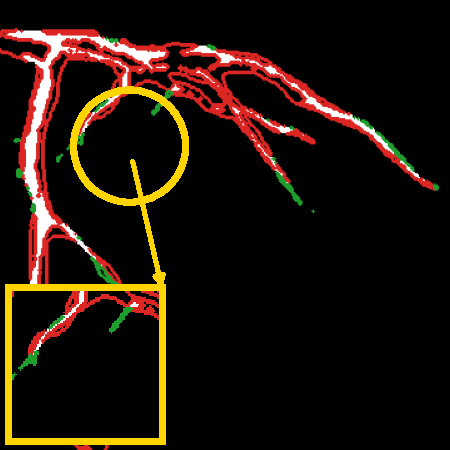
\includegraphics[width=\PW]{../img/dcd_fig6/fig5x6/r01_unet.pdf} & 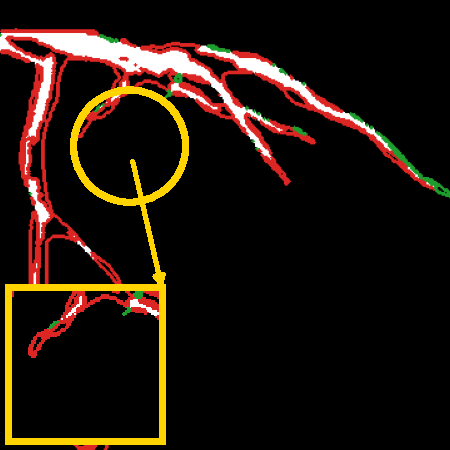
\includegraphics[width=\PW]{../img/dcd_fig6/fig5x6/r01_samocta.pdf} & 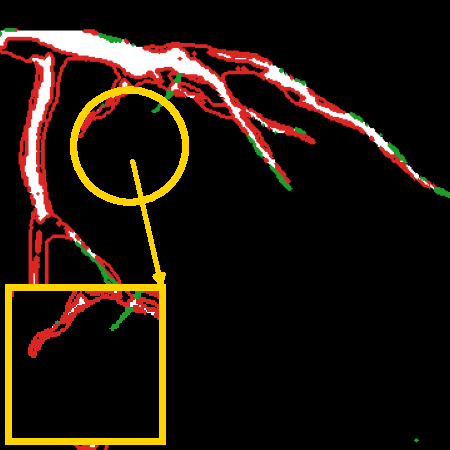
\includegraphics[width=\PW]{../img/dcd_fig6/fig5x6/r01_cwsam.pdf} & 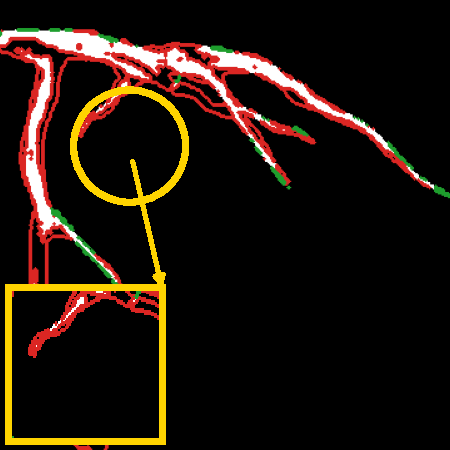
\includegraphics[width=\PW]{../img/dcd_fig6/fig5x6/r01_sacm.pdf} & 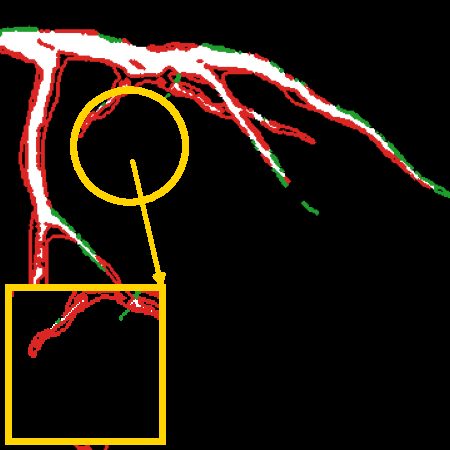
\includegraphics[width=\PW]{../img/dcd_fig6/fig5x6/r01_dcd.pdf} \\[1.5pt]
\makebox[\LabelW][c]{\rotatebox{90}{\scriptsize XCAD}} & 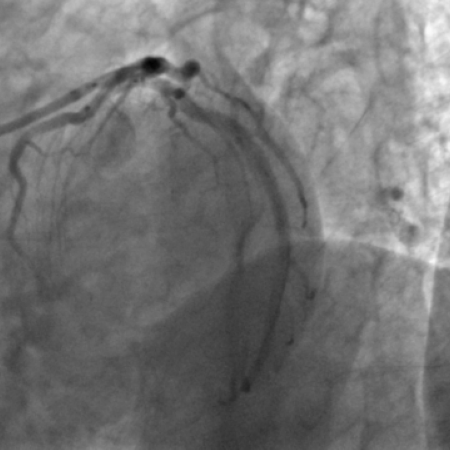
\includegraphics[width=\PW]{../img/dcd_fig6/fig5x6/r02_gt.pdf} & 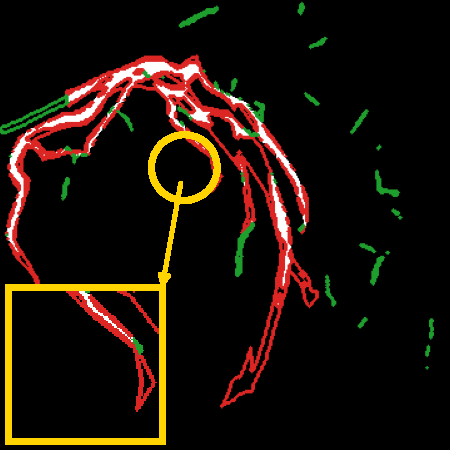
\includegraphics[width=\PW]{../img/dcd_fig6/fig5x6/r02_unet.pdf} & 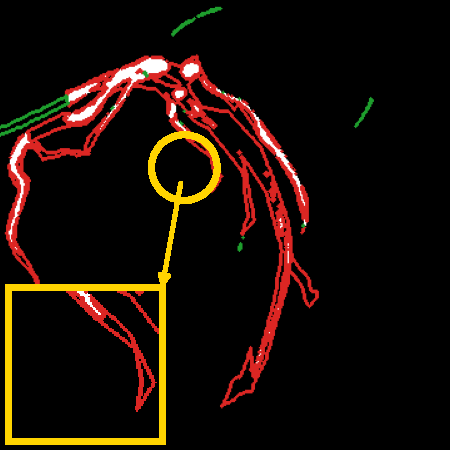
\includegraphics[width=\PW]{../img/dcd_fig6/fig5x6/r02_samocta.pdf} & 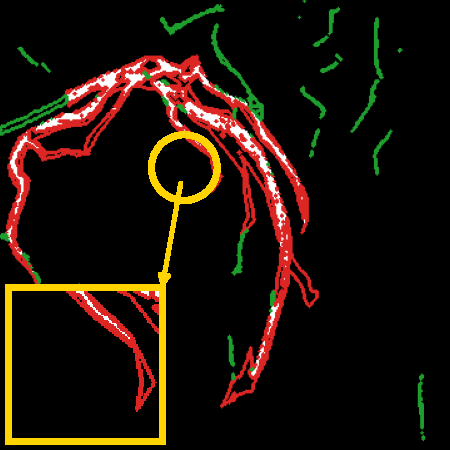
\includegraphics[width=\PW]{../img/dcd_fig6/fig5x6/r02_cwsam.pdf} & 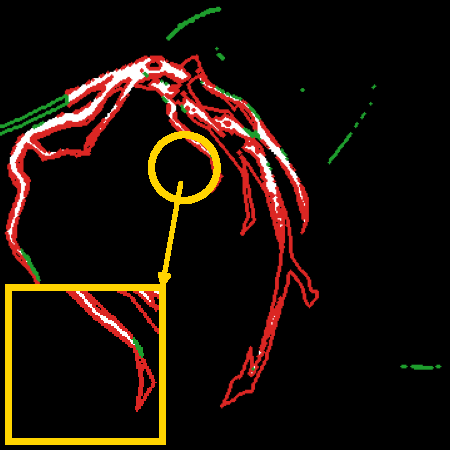
\includegraphics[width=\PW]{../img/dcd_fig6/fig5x6/r02_sacm.pdf} & 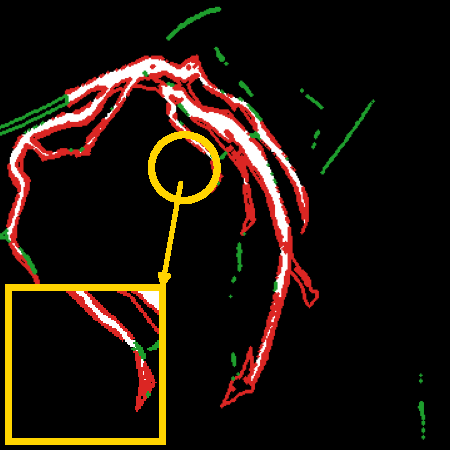
\includegraphics[width=\PW]{../img/dcd_fig6/fig5x6/r02_dcd.pdf} \\[1.5pt]
\makebox[\LabelW][c]{\rotatebox{90}{\scriptsize DeepCrack}} & 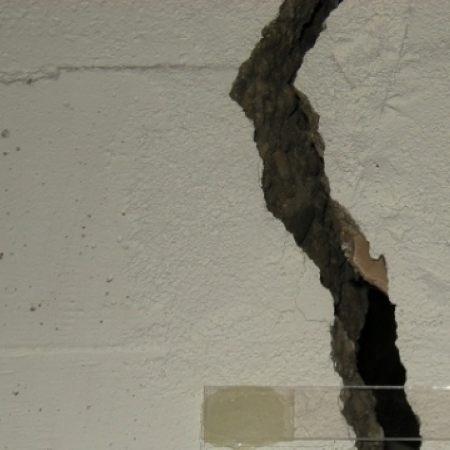
\includegraphics[width=\PW]{../img/dcd_fig6/fig5x6/r03_gt.pdf} & 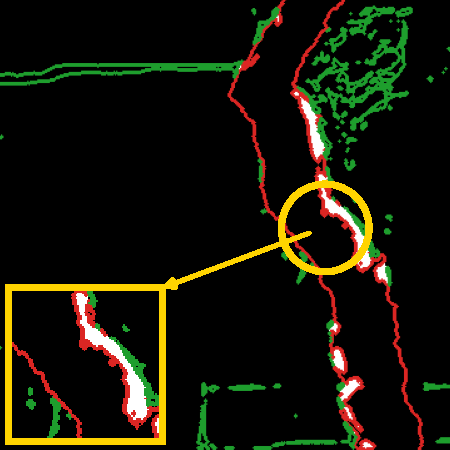
\includegraphics[width=\PW]{../img/dcd_fig6/fig5x6/r03_unet.pdf} & 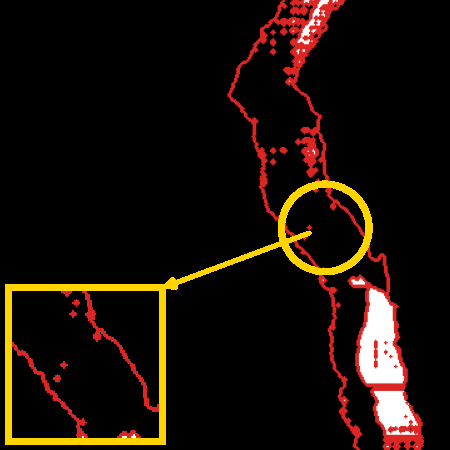
\includegraphics[width=\PW]{../img/dcd_fig6/fig5x6/r03_samocta.pdf} & 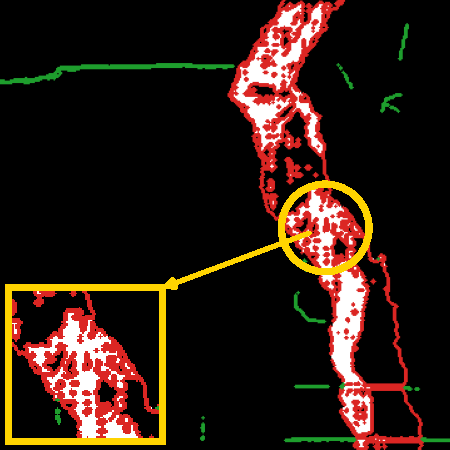
\includegraphics[width=\PW]{../img/dcd_fig6/fig5x6/r03_cwsam.pdf} & 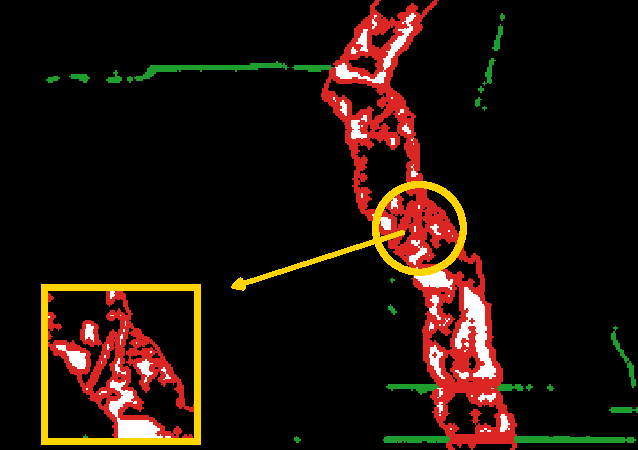
\includegraphics[width=\PW]{../img/dcd_fig6/fig5x6/r03_sacm.pdf} & 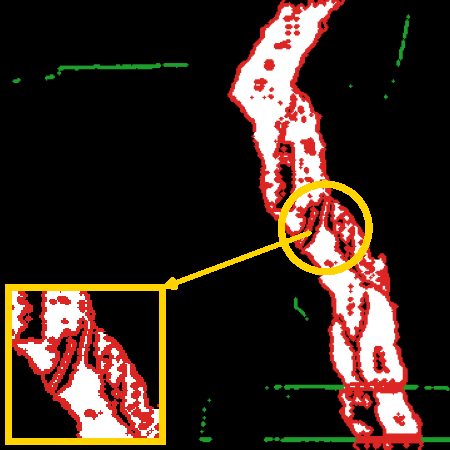
\includegraphics[width=\PW]{../img/dcd_fig6/fig5x6/r03_dcd.pdf} \\[1.5pt]
\makebox[\LabelW][c]{\rotatebox{90}{\scriptsize CHCrack5k}} & 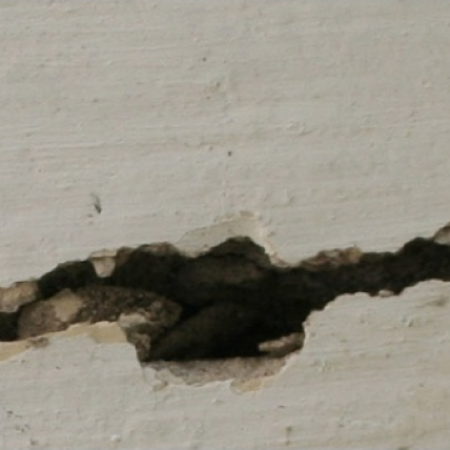
\includegraphics[width=\PW]{../img/dcd_fig6/fig5x6/r04_gt.pdf} & 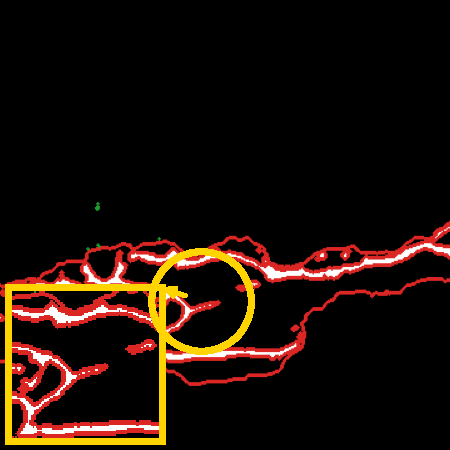
\includegraphics[width=\PW]{../img/dcd_fig6/fig5x6/r04_unet.pdf} & 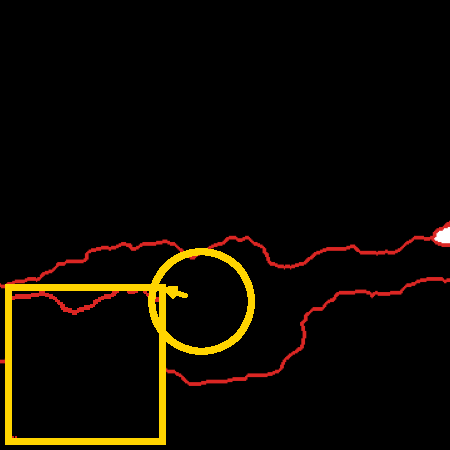
\includegraphics[width=\PW]{../img/dcd_fig6/fig5x6/r04_samocta.pdf} & 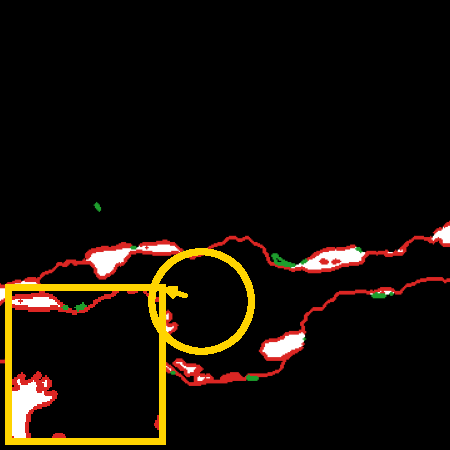
\includegraphics[width=\PW]{../img/dcd_fig6/fig5x6/r04_cwsam.pdf} & 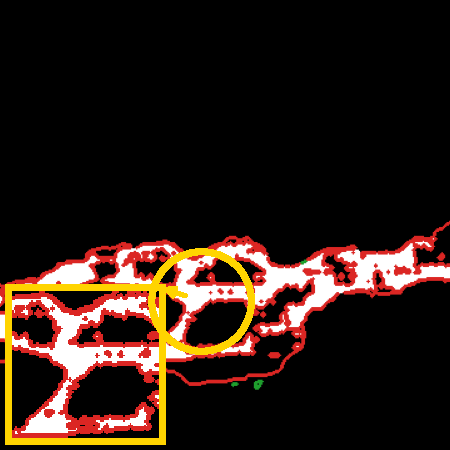
\includegraphics[width=\PW]{../img/dcd_fig6/fig5x6/r04_sacm.pdf} & 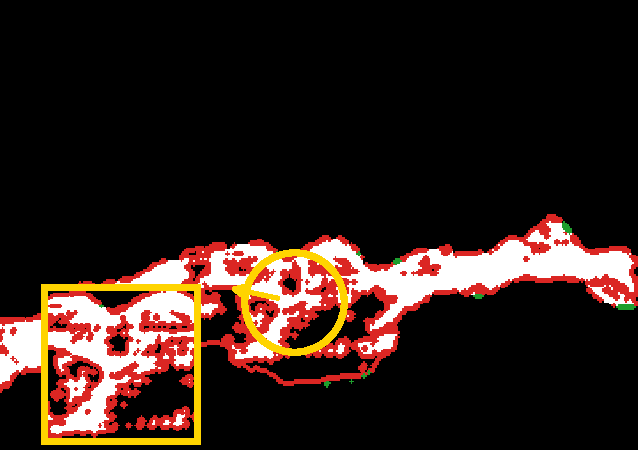
\includegraphics[width=\PW]{../img/dcd_fig6/fig5x6/r04_dcd.pdf} \\[1.5pt]
\makebox[\LabelW][c]{\rotatebox{90}{\scriptsize HRF}} & 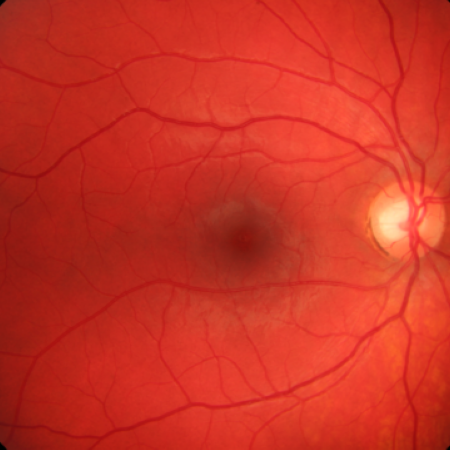
\includegraphics[width=\PW]{../img/dcd_fig6/fig5x6/r05_gt.pdf} & 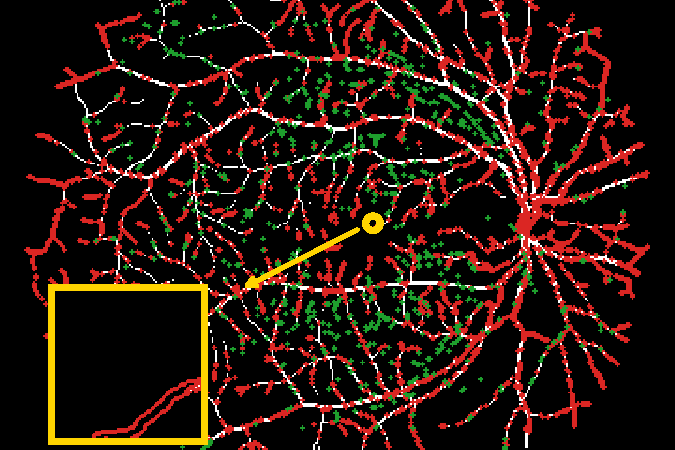
\includegraphics[width=\PW]{../img/dcd_fig6/fig5x6/r05_unet.pdf} & 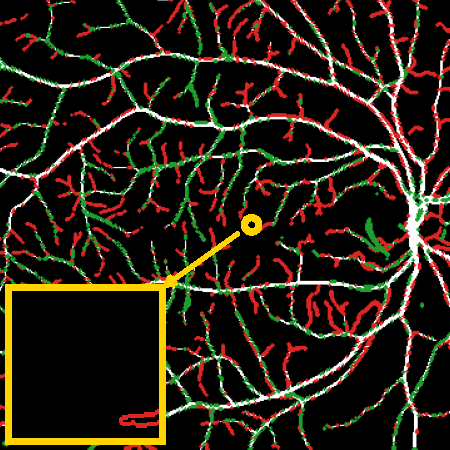
\includegraphics[width=\PW]{../img/dcd_fig6/fig5x6/r05_samocta.pdf} & 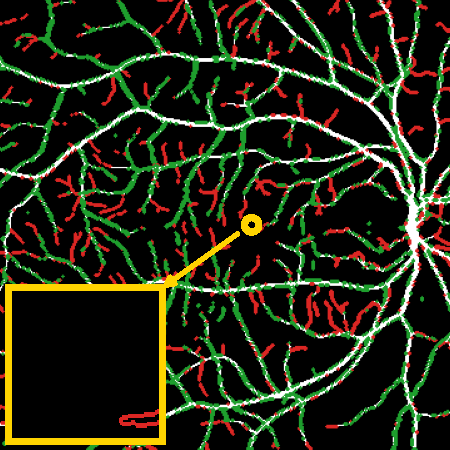
\includegraphics[width=\PW]{../img/dcd_fig6/fig5x6/r05_cwsam.pdf} & 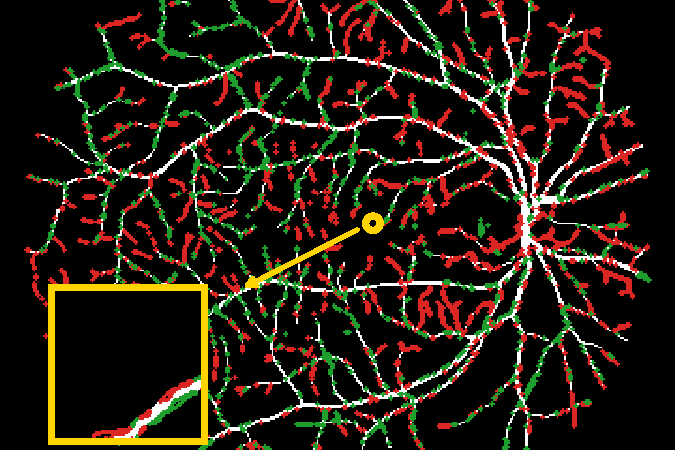
\includegraphics[width=\PW]{../img/dcd_fig6/fig5x6/r05_sacm.pdf} & 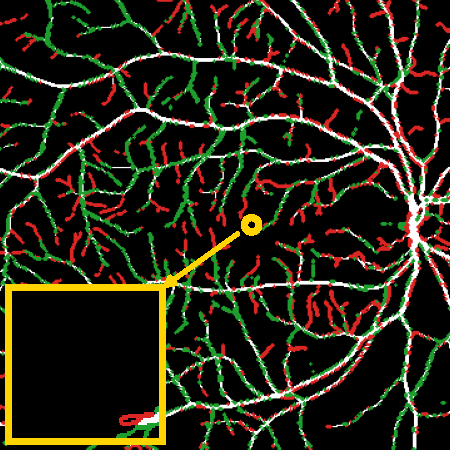
\includegraphics[width=\PW]{../img/dcd_fig6/fig5x6/r05_dcd.pdf} \\[1.2em]
\makebox[\LabelW]{} & \makebox[\PW][c]{\scriptsize Raw} & \makebox[\PW][c]{\scriptsize U-Net} & \makebox[\PW][c]{\scriptsize SAM-OCTA} & \makebox[\PW][c]{\scriptsize CWSAM} & \makebox[\PW][c]{\scriptsize SACM} & \makebox[\PW][c]{\scriptsize \textcolor{blue!60!black}{\textbf{Ours}}} \\
\end{tabular}
\caption{Qualitative comparison of Ours (DCD) with four baselines on five representative curvilinear datasets. The first column shows the raw input. In the prediction panels, white denotes true positives, red outlines false negatives, and green outlines false positives; black denotes background. Yellow insets magnify the same local region in each prediction column.}
\label{fig:dcd_showcase}
\end{figure}
